\section{Decentralized Structured Algorithms}
\label{section:structured}

This section focuses on the structured P2P architectures. The following
paragraphs contain a thorough discussion and analysis of the algorithms proposed
in the literature for dealing with the topology mismatch problem in such
architectures. In structured P2P systems, the construction of the routing tables
in every participating node determines the efficiency of message forwarding.
Therefore, routing tables that represent the underlying physical structure well
can achieve increased performance. For this reason, the proposed methods for
topology mismatch problem basically use different levels of proximity
information to optimize them towards this direction. The algorithms are here
categorised based the previous work done by
\cite{castro_proximitydht_2002,castro_topawareroute_2002,ratnasamy_openq_2002}.

%{\sethlcolor{yellow}\hl{HA:  Talk about Tapestry, Pastry, CAN and Chord briefly here!}}

%%%%%%%%%%%%%%%%%%%%%%%%%%%%%%%%%%%%%%%%%%%%%%%%%%%%%%%%%%%%%%%%%%%%%%%%%%%%%%%%
%%%%%%%%%%%%%%%%%%%%%%%%%%%%%%%%%%%%%%%%%%%%%%%%%%%%%%%%%%%%%%%%%%%%%%%%%%%%%%%%
\subsection{Geographic Layout}
%%%%%%%%%%%%%%%%%%%%%%%%%%%%%%%%%%%%%%%%%%%%%%%%%%%%%%%%%%%%%%%%%%%%%%%%%%%%%%%%
%%%%%%%%%%%%%%%%%%%%%%%%%%%%%%%%%%%%%%%%%%%%%%%%%%%%%%%%%%%%%%%%%%%%%%%%%%%%%%%%

Inside geographic layout category fall those kind of methods which practically
position physically close by nodes together in the application space as well.
This is done by adjusting and maintaining the routing tables of all involved
peers accordingly by exploiting proximity information that describe the overall
geographic positioning of the peer nodes. One popular method for detecting and
constructing a geographic view of the underlying network is the use of well
established servers dedicated to landmarking the physical space, pretty much as
discussed in Section \ref{sec:landmark} of landmark based proximity in the
unstructured P2P networks. The same disadvantages of difficult and inaccurate
positioning and the cost of deploying and maintaining these landmarks apply in
this case as well.
% TODO: maybe a discussion sentence bellow
Even though managing the overlay structure based on the geographic layout of the
nodes improves the query efficiency of the system, on the other hand, it tends
to create hotspots, and the needed failure resilience is undermined by the fact
that close by nodes are more likely to suffer collective failures.

%%%%%%%%%%%%%%%%%%%%%%%%%%%%%%%%%%%%%%%%%%%%%%%%%%%%%%%%%%%%%%%%%%%%%%%%%%%%%%%%
\paragraph*{\bf Global Soft-State}

\begin{figure*}
\centering
  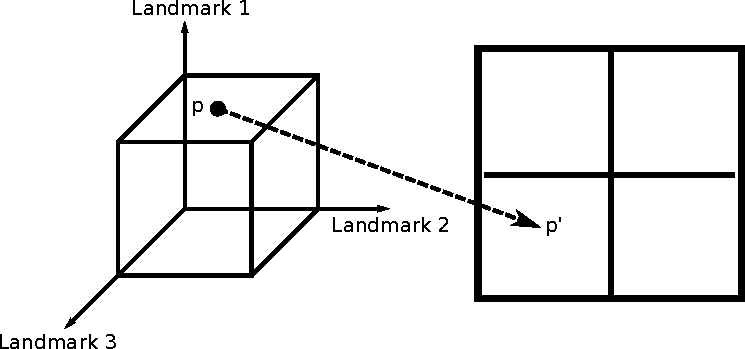
\includegraphics[scale=0.8]{img/algorithms/global_softstate}
\caption{(left) Position of $p$ in the space of $3$ landmarks. (right) Position
of $p$ on the map.}
\label{fig:global_softstate}
\end{figure*}

\textit{Global Soft-State} \cite{xu_globstate_2003} builds a global map to help
choose shorter routing paths, combining the landmark binning method and small
scale distance probes to reveal the proximity properties of the underlying
network to the overlay. Figure \ref{fig:global_softstate} presents the landmark
space and the mapping of the position of the nodes. This global view of the
state is made available to all nodes in order to help them find the best way to
route their messages. \textit{Global Soft-State} operates in two main stages,
generation and use of the proximity information. For generating the proximity
information a hybrid approach is proposed, which uses landmark clustering as a
preprocessing step in order to select a number of potential nearest neighbour
candidates and then refine the selection by incorporating a
round-trip-time-based scheme to ultimately choose the closest node. For using
the proximity information, the algorithm chooses a different path from the
classic gossiping approaches for constructing and maintaining the overlay. It is
based on landmark clustering for strategic placement of proximity information on
the overlay enabling any node to access such information using a landmark number
that reflects its physical position in the network. For various logical
regions\footnote{This might be a high-order zone in the eCAN\cite{xu_ecan_2002}
context or a set of nodes sharing a particular prefix in overlays such as
Pastry.} maps of physical information are built and published where each node
may appear in a maximum of $log\left( N \right)$ such maps. To dynamically adapt
to changing network conditions, a node subscribes to relevant \emph{soft states}
that utilize a notification system in order to initialize any necessary
neighbour re-selection.

Maintaining several host states at different layers, makes any content migration
costly. Additionally, the method does not make any continuing effort to remap
the overlay structure after a node successfully joins, in order to adapt its
state to any condition change. Although this approach greatly reduces the
routing latency to far nodes, it is unable to dynamically identify nodes that
are close to routers and gateways in order to construct the secondary overlay.
Nevertheless, static recognition of such nodes is currently done based on BGP
reports and pre-chosen landmarks, sacrificing the self-organising attribute of
traditional DHTs.

%%%%%%%%%%%%%%%%%%%%%%%%%%%%%%%%%%%%%%%%%%%%%%%%%%%%%%%%%%%%%%%%%%%%%%%%%%%%%%%%
\paragraph*{\bf Mithos}
\textit{Mithos} \cite{waldvogel_mythos_2003} is a P2P protocol which
incorporates directed incremental probing to find near optimal node placement,
and is classified by its authors as an integration of geographic layout and
proximity routing overlay optimization methods.

The bootstrap phase of \textit{Mithos} starts with a subset of existing members
as the first set of candidates, and while the iteratively closest nodes are
detected by probing the neighborhood, the candidate neighbor list is updated. In
order to avoid a local minima \textit{Mithos} probes all the neighbours within a
two hop distance from the current minimum before concluding the process.

After finding its first neighbour, the newcomming peer is assigned an ID using
information gathered during the iterative neighbour selection phase. Virtual
coordinates are assigned to the newcomming peer by using the distances of two
closest nodes and their neighbours, so that Euclidean distances between the node
and all known hosts predict the network latency between
them\cite{cox_vivaldi_2004}.  The benefit of these synthetic coordinates are
that they are explicitly used as the node's ID, and distance computations among
nodes can be done in ID space without requiring physical measurements.

The last step of the algorithm is the interconnection among neighbours.
\emph{Mithos} uses a \emph{quadrant}-based mechanism according to which each
node establishes a link to the closest neighbour in each quadrant. During
forwarding, the next hop is performed towards a neighbour in the same quadrant
as the final destination. The newcoming node may not know of other neighbours
in all quadrants, therefore, the node first identifies neighbours in all
quadrants using a mechanism based on ideas similar to a perimeter
walk\footnote{Used in Greedy Perimeter Stateless Routing (GPSR) protocol.} and
then improves the results using parallel path processing by taking into account
further geometric properties of node relationships.

One major limitation of \textit{Mithos} is that the protocol cannot handle
dynamic arrivals and removals from the network, as is happens in mobile
networks.

%%%%%%%%%%%%%%%%%%%%%%%%%%%%%%%%%%%%%%%%%%%%%%%%%%%%%%%%%%%%%%%%%%%%%%%%%%%%%%%%
\paragraph*{\bf LAPTOP}
\emph{LAPTOP} \cite{wu_laptop_2007},  organises the overlay into a tree-based
hierarchy with main focus on reducing hops during message routing as well as
minimizing maintenance overhead. Additionally, a caching scheme is also
incorporated so as to further reduce routing table update costs. The authors
theoretically show that in \textit{LAPTOP} routing path length is bounded by
$O(log_d N)$ and node joining and leaving in the overlay network is bounded by
$O\left( d log_d N \right)$ hops in a balanced overlay tree, where $N$ is the
number of nodes, and $d$ is the maximum degree of each node. \textit{LAPTOP}
implements the geographical layout approach  and constructs a geographical
layout in a self-organizing and efficient fashion, by estimating the
round-trip-times to a small number of nodes in the overlay network in order to
make them roughly aware of their physical distances among them.

Each node is assigned an address in a dotted format (e.g 1.3.4). Each octet
ranges from $1$ to $d$, where $d$ is the maximum degree of the nodes. The
assignment process is done by appending a unique octet to the address of each
nodes
parent, while root node is assigned address 1.  The routing scheme is similar to
the longest-prefix IP matching scheme. At each forwarding hop, any message
travels up the tree until the first common ancestor of both source and
destination nodes is reached and then starts descending to arrive to its target.
During tree traversals, special entries in the routing tables, called
\emph{routing cache}, are maintained in order to increase routing efficiency and
achieve finer load balance. Caching enables a node to forward a message to a
better longest-prefix match than that of its direct ancestor making a larger,
quicker and more cost effective step through the overlay and toward the
destination. To improve scalability, the number of children nodes and the size
of the routing cache are limited.  In terms of overlay maintenance, LAPTOP
incorporates a simple \emph{heartbeat}-based technique where each parent node is
responsible for monitoring its children.  At join process the newcomming node is
assigned its level label as well as its address by its parent node. Additionally
it initializes its routing table (with normal and caching entries) as it
traverses the overlay in search for its parent node.  During a graceful
departure, the referred node checks for children in the overlay. If it does not
have any, it simply notifies its parent and leaves. If it has, it selects the
child node with the lowest round-trip-time to it in order to take its place so
that the locality property is preserved.

%%%%%%%%%%%%%%%%%%%%%%%%%%%%%%%%%%%%%%%%%%%%%%%%%%%%%%%%%%%%%%%%%%%%%%%%%%%%%%%%
%%%%%%%%%%%%%%%%%%%%%%%%%%%%%%%%%%%%%%%%%%%%%%%%%%%%%%%%%%%%%%%%%%%%%%%%%%%%%%%%
\subsection{Proximity Routing}
%%%%%%%%%%%%%%%%%%%%%%%%%%%%%%%%%%%%%%%%%%%%%%%%%%%%%%%%%%%%%%%%%%%%%%%%%%%%%%%%
%%%%%%%%%%%%%%%%%%%%%%%%%%%%%%%%%%%%%%%%%%%%%%%%%%%%%%%%%%%%%%%%%%%%%%%%%%%%%%%%

Proximity routing does not require routing tables to be built using any
knowledge about network proximity. On the other hand it exploits such knowledge
in order to choose the best next hop during routing a message. This approach
balances between choosing the node that will further progress the routing
towards the destination and choosing the closest entry in the routing table, in
terms of network proximity.
% TODO: looks like discussion material
Thus, it is relatively less effective than
geographical layout when applied to CAN(-like) implementations. Moreover, the
technique has been incorporated into a version of Chord causing an increase on
the overhead of node joins and the size as well as maintenance cost of finger
tables.
%
%\cite{dabek_cfs_2001} proposes a server selection scheme for the Chord DHT, on
%the domain of proximity routing selection. In \emph{CFS}, each node predicts
%the entire lookup latency as a function of the total number of nodes and the
%average overlay next routing peer. The problem is that it is very difficult to
%have a clear picture on the total number of nodes and the average hop latency
%from the local. This leads to rough estimations that consequently decreases
%overall performance.
%
The methods that use proximity routing and their details are listed below.

%%%%%%%%%%%%%%%%%%%%%%%%%%%%%%%%%%%%%%%%%%%%%%%%%%%%%%%%%%%%%%%%%%%%%%%%%%%%%%%%
\paragraph*{\bf Proximity in Kademlia}
Before discussing {\em Proximity in Kademlia}, it would be helpful to briefly
summarize the highlights about the {\em Kademlia} protocol. {\em Kademlia}
\cite{maymounkov_kademlia_2002} is a distributed hash table (DHT) based
protocol for P2P networks, which uses an iteration based lookup algorithm. The
protocol uses the standard $160$ bit ID system for nodes and locates the nodes
in a prefix binary tree, where IDs are used as prefixes. The iterative lookup
operations are done over this prefix binary tree, which converges to logarithmic
lookup times. The ID's are assigned randomly, therefore in Kademlia, there is no
proximity control, which results in inefficient use of the underlying network
during lookup and retrieve operations.

{\em Proximity in Kademlia} \cite{kaune_pkad_2008} introduces proximity controls
over the base Kademlia protocol to optimize the underlying network usage of the
protocol. The authors define an abstract {\em underlay metric} that calculates
the suitability of establishing a communication link between peers as a cost
function, based on the used proximity criteria (RTT, ISP locality, etc.).
{\em Proximity in Kademlia} adapted both {\em proximity routing} and {\em
proximity neighbour selection} overlay optimization algorithms for controlling
proximity. Therefore, we categorize the protocol only in this section, and skip
the discussion in the further {\em proximity neighbour selection} section
(Sec.\ref{sec:pns}). {\em Proximity in Kademlia} also uses the MaxMind GeoIP
database\footnote{MaxMind Geolocation Technology. http://www.maxmind.com} to
detect the proximity information of a given peer based on its region, country,
or ISP location, and use this information to form clusters of nearby peers. One
other method {\em Proximity in Kademlia} uses is the Vivaldi
\cite{cox_vivaldi_2004} protocol. However, authors report that clustering
approach performs better than Vivaldi protocol based on their experiments.
Authors also report that {\em Proximity routing} protocol successfully worked
with the Kademlia protocol and improved the locality of the connections over
peers.

%%%%%%%%%%%%%%%%%%%%%%%%%%%%%%%%%%%%%%%%%%%%%%%%%%%%%%%%%%%%%%%%%%%%%%%%%%%%%%%%
\paragraph*{\bf CHOord considering Proximity on IPv6 (CHOP6)}
\textit{CHOP6} \cite{morimoto_chop6_2007} is designed based on the
\textit{Chord} protocol. \textit{CHOP6} roughly estimates the proximity among
nodes by exploiting the IPv6 address format and RTT information if available.
The proximity estimation is achieved by introducing a 64-bit ID scheme in which
the least significant bit part is the IPv6 global routing prefix and thus
enabling a longest prefix match scheme. The protocol is designed based on the
observation that it is possible to estimate a node's geographical location by
simply examining the upper 32-bits of its IPv6 address. Moreover, similar to
\textit{Chord}, \textit{CHOP6} uses a finger table, whose entries hold more than
one candidate node.

%%%%%%%%%%%%%%%%%%%%%%%%%%%%%%%%%%%%%%%%%%%%%%%%%%%%%%%%%%%%%%%%%%%%%%%%%%%%%%%%
\paragraph*{\bf Chord6}
\emph{Chord6} \cite{xiong_chord6_2005} is another \textit{Chord} variant that
tries to exploit the hierarchical features of IPv6 in order to create a
substrate that reduces interdomain traffic between service providers.
\textit{Chord6} is based on the original Chord protocol, and the main difference
from the original protocol is in the identifier definition. Therefore, the
approach can be easily portable to other DHTs such as CAN, Pastry and Tapestry.
In Chord6 the identifier contains two parts: the higher bits are obtained by
hashing the node's IPv6 address prefix of specific length, while the remaining
lower bits are the hash value of the rest of that IPv6 address. As a result of
this assignment, nodes in a domain will be mapped onto a continuous key space on
the overlay network, which avoids unnecessary message forwarding across
different service providers, thus minimizing overall routing cost.

%%%%%%%%%%%%%%%%%%%%%%%%%%%%%%%%%%%%%%%%%%%%%%%%%%%%%%%%%%%%%%%%%%%%%%%%%%%%%%%%
%%%%%%%%%%%%%%%%%%%%%%%%%%%%%%%%%%%%%%%%%%%%%%%%%%%%%%%%%%%%%%%%%%%%%%%%%%%%%%%%
\subsection{Proximity Neighbour Selection}\label{sec:pns}
%%%%%%%%%%%%%%%%%%%%%%%%%%%%%%%%%%%%%%%%%%%%%%%%%%%%%%%%%%%%%%%%%%%%%%%%%%%%%%%%
%%%%%%%%%%%%%%%%%%%%%%%%%%%%%%%%%%%%%%%%%%%%%%%%%%%%%%%%%%%%%%%%%%%%%%%%%%%%%%%%

\textit{Proximity Neighbour Selection} constructs the routing tables using
proximity knowledge. The proximity information used in this method is different
than the landmark based systems described in the \textit{Geographic Layout}
section, as time-to-live values between nodes, or directly node ID prefixes are
used to detect proximity.  Tapestry, Pastry, and CAN successfully implemented
the proximity into their algorithms by using this approach.  The routing
protocol in Pastry is based on longest node ID prefix matching, while CAN uses
RTT values to detect close by nodes. \cite{castro_proximityp2p_2002}  reports
that proximity neighbour selection as an effective proximity based method.
Proximity Neighbor Selection based algorithms are described in detail below.


%%%%%%%%%%%%%%%%%%%%%%%%%%%%%%%%%%%%%%%%%%%%%%%%%%%%%%%%%%%%%%%%%%%%%%%%%%%%%%%%
\paragraph*{\bf DHT-PNS}
Chord-DHT-PNS \cite{hancong_pnsbased_2006} implements proximity neighbour
selection on top of the Chord DHT. The main goal is to use proximity information
to group physically close by nodes as neighbours in the DHT table. In order to
detect proximity, virtual network coordinates of peers are used, by using the
Vivaldi protocol \cite{cox_vivaldi_2004}. The virtual coordinates are then used
by the nodes to map to identifier space in the DHT. The space is partitioned
using a \emph{concentric circle clustering scheme} where successive cycles of
radiuses $\rho$, $2\rho$, $3\rho$ and so on, are constructed. Then the formed
annuluses are divided into $2\chi-1$ \emph{sectors}, where $\chi$ denotes the
sequence number of the annulus starting from $\chi = 1$ for the centre cycle. It
is proved in the paper, that this way each sector occupies the same area as does
the center cycle. Assuming uniform node distribution, this characteristic,
favours a more load balanced clustering operation. Every sector in this $2D$
coordinate space is mapped to a unique \emph{region} in the DHT space forming a
multi-layer node identifier space.  Thus, any nodes that belong to the same
sector, are mapped to the same region as well, preserving their proximity
relationship unveiled by the use of the Vivaldi protocol. The individual pieces
are mapped to the identifier space uniquely, allowing logarithmic lookup
operations with high probability on Chord.

%%%%%%%%%%%%%%%%%%%%%%%%%%%%%%%%%%%%%%%%%%%%%%%%%%%%%%%%%%%%%%%%%%%%%%%%%%%%%%%%
\paragraph*{\bf IP-based Clustering (IPBC)}
Proximity neighbour selection algorithms use probing and other techniques
to detect proximity. However, such methods are either not precise enough, or
overload the network. \emph{IP-based clustering}
\cite{karwaczynski_ipbc_2007} is a proximity neighbour selection based
algorithm in which the authors propose to use the IP address prefixes (16 bit
for IPv4) in order to detect proximity.  \cite{freedman_iploc_2005} states that
$97\%$ of prefixes larger than $24$ bits belong to a single geographical
location. However, using less number of bits creates less precise results and
more number of bits increase the burden on the network and reduce the possible
number of neighbours. Therefore, a careful selection is required in terms of
performance/accuracy tradeoff. The {\em IP-based Clustering} generates a key and
its prefix and stores the later in the DHT itself, so that any newly joining
nodes with the same IP prefix can query it and identify all the
neighbours with the same one relatively easily. Nodes periodically update
their entries in the DHT by removing those who leave, or those who has been
timed out with no further activity detected from the node.

%%%%%%%%%%%%%%%%%%%%%%%%%%%%%%%%%%%%%%%%%%%%%%%%%%%%%%%%%%%%%%%%%%%%%%%%%%%%%%%%
\paragraph*{\bf Cone}
\textit{Cone}\cite{wang_cone_2007} extends Chord using proximity neighbour
selection topology optimization algorithm. The proximity information is
generated using landmarks and round-trip-time-based distances to landmarks.
\textit{Cone} uses a two-layered identifier space. The first, named Chord-layer
identifier, denoted as $Id_{Chord}$, is the same as in Chord. The second is the
Cone-layer identifier, $Id_{Cone}$ which is constructed by two component
identifiers. The first, known as \emph{group identifier (gid)} denotes a
relevant group the node belongs to while the second, namely \emph{local
identifier (lid)} indicates the local identifier within the group. The group
concept, which is introduced here, is a way of dividing nodes according to a
common $Id_{Chord}$ prefix.  The structure of a Cone overlay, retains the
Chord's circular topology. The difference lies on the fact that, now, two rings
are created. A big ring, where nodes with the same \emph{gid} are arranged at
each position. Each of these positions are a smaller ring for the particular
group's \emph{lid}s. The routing is achieved in both clockwise and
counter-clockwise directions in the big-ring, for which two routing tables are
maintained, namely \emph{front} and \emph{back} finger tables. Entries in these
tables, display physical network proximity with the current node. Moreover, a
third table called \emph{group} maintains information about other online peers
within the current node's group in a way that entries are now close in the ID
space.

%%%%%%%%%%%%%%%%%%%%%%%%%%%%%%%%%%%%%%%%%%%%%%%%%%%%%%%%%%%%%%%%%%%%%%%%%%%%%%%%
\paragraph*{\bf SAT-Match: Self-Adaptive Topology Matching}

\begin{figure}[ht]
\centering
\subfigure[Example physical topology of nodes.] {
  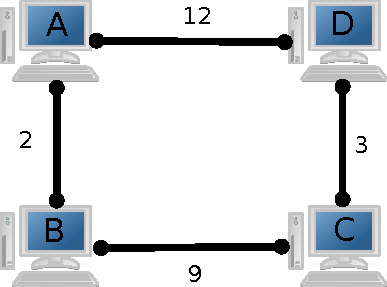
\includegraphics[scale=0.6]{img/algorithms/SAT_match}
  \label{figure:sat_match:before}
}\qquad\qquad
\subfigure[(left) A jumps to B in order to match the logical topology to the
physical. (right) State of the logical topology after the jump.] {
  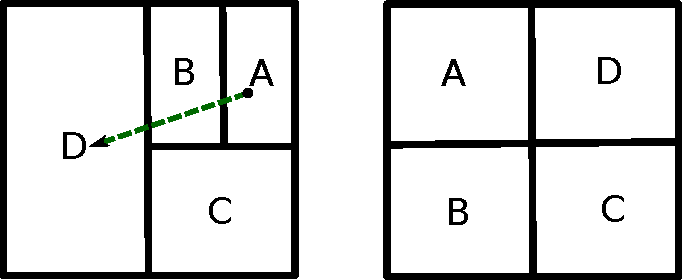
\includegraphics[scale=0.6]{img/algorithms/SAT_match2}
  \label{figure:sat_match:after}
}
\caption{The SAT-Match algorithm.}
\label{figure:sat_match}
\end{figure}

\textit{SAT-Match} \cite{ren_satmatch_2004} is a protocol that specifically
tries to solve the topology mismatch problem by mapping the overlay network as
close as possible to the physical one. Even though no theoretical proof is
given, valid results are obtained and demonstrated through experimentations.
Similar to the other approaches in the proximity neighbour selection,
\textit{SAT-Match} uses probing to detect close by peers and obtain proximity
information. However, as an additional feature, \textit{SAT-Match} peers can do
selective jumps to adjust their positioning in the DHT, if it reduces the stretch
of its one-hop neighbourhood. Figure~\ref{figure:sat_match} demonstrates the
selective jump on an example topology. The stretch is defined as the ratio
between the average logical and physical latency of a link. It is reported that,
due to the selective jumps, the \textit{SAT-Match} achieves $40\%$ reduction in
link stretch, and when used with the \textit{Landmark Binning} approach (see
Sec. \ref{sec:landmark_binning}), the reduction rate increases up to $60\%$.
For dynamic environments, with frequent node arrival and leave,
\textit{SAT-Match} scales much better than \textit{Mithos}, due to its self
adaptation mechanism and selective jumps.

\emph{SAT-Match} uses a small TTL value for the probing messages in order to
reduce redundancy\cite{jiang_lightflood_2008}. This process begins as soon as
the node joins the network using a DHT mechanism. Each probing message contains
information about the source and a small TTL value. The recipient of such a
message returns information about itself to the source and forwards the probing
message to its neighbours if the TTL is non-zero. The discovered nodes are
referred to as $TTL-k$ neighbourhood of the source node based on the $TTL$
distance to the source node.

Blindly selecting the peer with the smallest RTT as neighbour is, generally, not
the optimal decision to make in order to achieve global \emph{stretch} reduction.
In a structured scheme, when a node jumps to connect to a physically close node,
it may need to connect to other distant nodes to maintain the structure's
integrity, thus creating an overall increase in the overlay's \emph{stretch}.
The two nodes with the smallest RTT are then used in order to select one zone to
jump in this phase. The algorithm is as follows: The source node $S$ calculates
the stretch change of its $TTL-1$ neighbourhood and that of the $TTL-1$
neighbourhood of the first of the previously selected peers. These calculations
are made as if the jump has been made. If the stretch reduction is over a
predefined threshold the jump is performed, otherwise the second selected
candidate is picked and the same computations are performed. If again, the
threshold is not met, then no jump is ultimately done. In case of a jump, this
is performed as a combination of \emph{leave} and \emph{join} operations, in the
CAN context.

%\begin{figure}[h!]
\hspace{-3ex}
\begin{center}
\footnotesize
%\begin{landscape}
\begin{longtable}{
|>{\columncolor[gray]{.7}}m{0.2\columnwidth}
|>{\columncolor[gray]{.9}}m{0.4\columnwidth}
|>{\columncolor[gray]{.8}}m{0.2\columnwidth}
|>{\columncolor[gray]{.9}}m{0.2\columnwidth}
%|>{\columncolor[gray]{.9}}m{0.1\columnwidth}
%|>{\columncolor[gray]{.8}}m{0.1\columnwidth}
%|>{\columncolor[gray]{.9}}m{0.1\columnwidth}
%|>{\columncolor[gray]{.8}}m{0.1\columnwidth}
|}
\caption{Decentralized Structured Algorithms}\label{fig:struct_compare_table}\\
\hline
\rowcolor[gray]{.5}
\textbf{Algorithm} & \textbf{Overlay structure} & \textbf{Base protocol} & \textbf{Scalability} \\
\hline
\endfirsthead
\multicolumn{4}{c}%
{\tablename\ \thetable\ -- \textit{Continued from previous page}} \\
\hline
\rowcolor[gray]{.5}
\textbf{Algorithm} & \textbf{Overlay structure} & \textbf{Base protocol} & \textbf{Scalability} \\
\hline
\endhead
\hline \multicolumn{4}{r}{\textit{Continued on next page}} \\
\endfoot
\hline
\endlastfoot

\hline
\textbf{Global Softstate} &
\textbf{Geographic layout} Uses first landmark clustering
then measures RTTs to identify close nodes &  &  \\

\hline
\textbf{Mithos} &
\textbf{Geographic layout} Uses nodes as topology landmarks and directed
incremental probing to optimize topology & & Scales well as all
operations are local ??? \\

\hline
\textbf{Self-Adaptive Topology Matching} &
\textbf{Proximity neighbour selection} Uses lightweight probing and
selective jumps to optimize the topology & CAN &  Better than Mithos \\

\hline
\textbf{Delay Aware P2P System} & \textbf{} & & \\

\hline
\textbf{VERSION OF CHORD - DHT-PNS} &
\textbf{Proximity neighbour selection} Uses Proximity Neighbour Selection and the Vivaldi
system & Chord  &  \\

\hline
\textbf{MAY OMIT- VERSION OF CHORD - Quasi-Chord} &
\textbf{Proximity based}  & Chord  &  \\

\hline
\textbf{LAPTOP} &
\textbf{Geographic layout} Hierarchical overlay structure  &  & routing path length $\log{_d N}$,
join/leave overhead $d\log{_d N}$ \\

\hline
\textbf{IP-Based Clustering} &
\textbf{Proximity neighbour selection} Proximity neighbour selection based on longest common
prefix of IP addresses &    &  \\

\hline
\textbf{CHOord considering Proximity on IPv6} &
\textbf{Proximity routing} Uses IPv6 address format to provide proximity &  Chord
 & Better than Chord \\

\hline
\textbf{Proximity in Kademlia} &
\textbf{Proximity routing} Applies  proximity neighbour selection (PNS) and proximity route selection (PRS)
to Kademlia & Kademlia &   \\

\hline
\textbf{Cone} &
\textbf{Proximity neighbour selection} Uses proximity neighbour selection (PNS) & Chord  & Better than Chord \\

\hline
\textbf{Dynamo} &  &  &  \\

\hline
\textbf{MAY OMIT-BADLY WRITTEN-PChord} &
\textbf{Proximity based}  &  Chord  & \\

\hline
\textbf{AChord} &  & & \\

\hline
\textbf{Chord6} &
\textbf{Proximity routing} Uses IPv6 hierarchical address format to cluster
topologically close nodes & Chord  &  \\

\hline
\end{longtable}
%\end{landscape}
\end{center}
\vspace{-2.5ex}
\vspace{-2.5ex}
%\label{fig:struct_compare_table}
%\end{figure}

%%%%%%%%%%%%%%%%%%%%%%%%%%%%%%%%%%%%%%%%%%%%%%%%%%%%%%%%%%%%%%%%%%%%%%%%%%%%%%%%
%%%%%%%%%%%%%%%%%%%%%%%%%%%%%%%%%%%%%%%%%%%%%%%%%%%%%%%%%%%%%%%%%%%%%%%%%%%%%%%%
\subsection{Discussion on the Algrithms for Structured Architectures}
%%%%%%%%%%%%%%%%%%%%%%%%%%%%%%%%%%%%%%%%%%%%%%%%%%%%%%%%%%%%%%%%%%%%%%%%%%%%%%%%
%%%%%%%%%%%%%%%%%%%%%%%%%%%%%%%%%%%%%%%%%%%%%%%%%%%%%%%%%%%%%%%%%%%%%%%%%%%%%%%%

In this section we presented the state of the art for the algorithms applied to
structured P2P systems. We categorised it based on their philosophy they
incorporated in order to alleviate the topology mismatch problem into overall
three categories following the previous work from
\cite{castro_proximitydht_2002,castro_topawareroute_2002,ratnasamy_openq_2002}
namely
\begin{inparaenum}[\itshape i\upshape)]
  \item geographic-layout-based,
  \item proximity-routing-based, and
  \item proximity neighbour selection based
\end{inparaenum}
. Following is a discussion on the above categories trying to point out the
advantages, disadvantages and novelties introduced by each and by all of them.
A quick overview can be seen in Table \ref{fig:struct_compare_table}.

In Section~\ref{section:structured}, we presented the state of the art
structured decentralized P2P algorithms in three different categories based on
their handling of the network structure to tackle the topology mismatch problem:
geographic layout based, proximity routing based, and proximity neighbour
selection based. In this section, we present a final discussion of all the
methods including the advantages, disadvantages, and novelties related to solve
the topology mismatch problem. Table~\ref{fig:struct_compare_table} presents an
overview of all the structured decentralized algorithms described earlier in
this section.

Structured P2P network algorithms use a global distributed hash table or a
prefix tree structure to uniquely lookup peers or their data in the overlay
network. As all the data is kept within the overlay, each node behaves as a
client and a server, therefore nodes join and leave according to rules
determined by the integrity of the global data structure. The main advantage of
the structured P2P topology is that by the help of the global data structure,
peers or their data can be found within the network even if there is only a
single copy of that item present. However, each node join and leave creates
maintenance overhead for the network due to updates required by the global data
structure, and for networks with frequent node arrivals and departures the
topology uses valuable network resources just to update the global structure.
Nodes join the network by using a key value, which determines the location and
the neighbourhood of the new node within the network. However, assigning
random key values to the newly inserted nodes creates non-optimal matching with
the underlying physical network topology, therefore, increasing the overhead of
the network even more. One solution for handling the topology mismatch problem
is to consider the proximity of the peers when generating the key and joining
the node to the network, so that nodes within the same network domains are
selected as peers, or neighbours, during the overlay topology construction. In
this chapter, we have described three such approaches to optimize the topology
matching problem: geographic layout, proximity routing and proximity neighbour
selection.

In geographic layout, nodes try to estimate the geographic positions of the
peers, and construct the DHT considering the proximity of the peers. Landmark
servers and RTT measurements are two popular methods, which can also be used in
conjunction, to discover physically close by peers over the network. However, as
discussed in Section \ref{sec:landmark_binning}, these methods do not always
give reliable estimates for the node positions over the internet. The landmark
servers are not self-organizing and have maintenance overheads. To serve a
P2P network with millions of peers, multiple landmark servers
distributed over the whole world is required, which is hard to manage. The RTT
measurements also can measure the delay between peers, but it is a greedy method,
which can result non-optimal overlay topologies especially if close by nodes
have low bandwidth connections among themselves.

Proximity routing does not discover or store proximity information for the
peers, however, during package forwarding, nodes that have lower latency to the
destination, or with a closer key to the destination is selected. As no
proximity information is used, the system is based on a greedy approach and it
usually selects low latency paths over the overlay, which maps to suboptimal
longer paths on the physical topology. For these obvious reasons, proximity
neighbour selection is generally considered as a superior method to proximity
routing, however, joint uses of these two protocols are also possible.

Proximity neighbour selection approach is similar to proximity routing, with an
exception that during forwarding, the proximity information of the peers are
also considered. Therefore, for each application, proximity information is
extracted and used during routing. Depending on the application, the proximity
information can be the node sharing the same prefix with the current node, or
TTL to detect close by neighbours. Tapstry and Pastry are two popular methods
implementing the proximity neighbour selection among others mentioned above in the
proximity neighbour selection section.